% !TEX root = MutationTestingSurvey.tex

\subsection{Data Modeling}
\label{sec:dataModeling}

Approaches performing data mutation often require a data model to drive mutations (e.g., to decide how to alters a specific chunk of data). 
However, some of the approaches do not require a data model. 
These approaches are the ones that perform low level changes (e.g., bit flips) or that combine multiple low level changes driven by the data collected at runtime (e.g., AFL ).
The main drawback of approaches that do not require a data model is that they can hardly be used in a mutation testing context.
Indeed, without additional information (e.g., a data model) it is not possible to determine what should be the expected effect of modifying a randomly selected portion of an input, in turn, it is not possible to determine if the mutated data should lead to a test failure, trigger a robustness feature of the SUT, or simply go unnoticed because it does not alter the behaviour of the software (e.g., because it alters bytes that are copied as is by a data processing system).

Three are the main solutions adopted for data modelling, the use of grammars~\cite{Godefroid:GrammarBasedFuzzying:2008,godefroid2012sage,bounimova2013billions}, the use of UML models~\cite{di2015evolutionary}, and the use of custom models~\cite{pham2016model,PeachFuzzer}.

\subsubsection{Data modeling with grammars}

Grammar-based approaches rely on a context-free grammar to specify the format of the data to be mutated. Grammars are used by fuzzying approaches that alter input files to perform robustness testing.
The main limitation of grammars is that they cannot be used to encode integrity constraints such as size-of, offset-of, length-of and checksums~\cite{pham2016model}. 

\subsubsection{Data modeling with UML models}

Approaches relying on UML models~\cite{di2015generating,di2015evolutionary} use class diagrams to capture the structure of inputs and outputs, expressions written with the Object Constraint Language (OCL)~\cite{OCL} to define relationships between the inputs and outputs, and UML stereotypes to capture a fault model driving the generation of test cases.
Figure~\ref{fig:dataModel} shows an example input data model~\cite{di2015evolutionary}.
The model captures the structure of a network transmission; UML classes represent elements that contain multiple fields, while UML attributes model elements that cannot be further decomposed. For example, it shows that each transmission consists of a sequence of \emph{Virtual Channel Data Units (VCDUs)}. Each \emph{VCDU} begins with a \emph{Header}, followed by a \emph{PacketZoneHeader} and a \emph{PacketZone} that may contain a sequence of \emph{Packets} (if the packet zone is active).
The \emph{VCDUs} in a transmission may belong to different virtual channels.
Associations are used to represent containment relationships. In Figure~\ref{fig:dataModel} the classes that model the VCDU and its Header are connected by an association.
Class attributes represent the transmitted binary information. For example, attribute \emph{sequenceCount} of class \emph{Packet} is used to store information about the packet order.
Stereotypes to capture the fault model of the system. 
%and are used to identify the fields that can be mutated to generate new inputs.
For example, 
the two stereotypes \emph{Identifier} and \emph{Measure} are used to indicate that these attributes should be modified using mutation operators specified for identifiers and measurements.


In the presence of UML models, constraints between inputs and outputs can be represented using OCL.
These constraints are used as an oracle to validate the execution of automatically generated test cases: a violated constraint indicates that the system under test does not produce the expected output. 
The use of OCL constraints enable engineers to represent information that cannot be captured with grammars.
%In the case of SES-DAQ, we use OCL constraints to model the error messages expected in the presence of specific faults in the input data.
For example, Figure~\ref{fig:costraint:firstHeader} shows an OCL constraint that states that the frame count of a VCDU should be greater by one than the frame count of the previous VCDU on the same virtual channel. Otherwise, an error event \emph{COUNTER\_JUMP} should exist in the system output log file. 

\begin{figure}[t!]
  \centering
    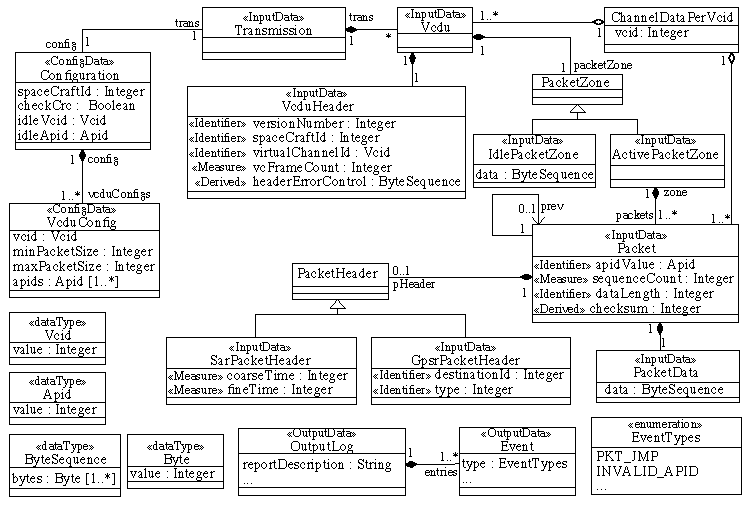
\includegraphics{images/classDiagramSmall}
      \caption{Simplified input data model taken from~\cite{di2015evolutionary}.}
      \label{fig:dataModel}
\end{figure}

\begin{figure}[t!]
\scriptsize
\begin{tabular}{p{0.1cm}p{8cm}}
1&\textbf{context} Vcdu \textbf{inv}:\\
2&\textbf{let}\\
3&\hspace{0.3cm}frameCount : Integer = self.header.vcFrameCount, \\
4&\hspace{0.3cm}vdcuIndex : Integer = self.virtualChannel.vcdu$\rightarrow$indexOf( self ), \\
5&\hspace{0.3cm}previous : Vcdu = self.virtualChannel.vcdu$\rightarrow$at( vcduIndex - 1 ),\\
6&\hspace{0.3cm}previousFrameCount : Integer = previous.header.vcFrameCount\\
7&\textbf{in} \\
8&\hspace{0.3cm}\textbf{if} previousFrameCount $<$ 16777215 \\
9&\hspace{0.6cm}\textbf{then} frameCount $<>$ previousFrameCount + 1 \\
10&\hspace{0.3cm}\textbf{else} previousFrameCount $=$ 16777215 and frameCount $<>$ 0 \textbf{endif}\\
11&\textbf{implies} \\
12&\hspace{0.3cm}VcduEvents.allInstances()\\
13&\hspace{1cm}$\rightarrow$exists(e $|$ e.eventType = $COUNTER\_JUMP$) \\
\end{tabular}
\caption{Input/output constraint for the \emph{COUNTER\_JUMP} error event.}
\label{fig:costraint:firstHeader}
\end{figure}


 
%The stereotype \emph{Derived} is used to tag class attributes that need to be derived from other attributes after every mutation, in order to prevent trivial inconsistencies (e.g. it is used to update the checksum field when other fields are mutated). 
%The stereotypes \emph{StreamClass} and \emph{StreamAttributes} are used to automate the loading of data from bytestreams.
% but are out of the scope of this paper (see~\cite{ICST15} for details).

The main limitation of UML based approaches is the lack of generalistic binary parsers capable of loading data as an instance of a UML class diagram. Existing approaches rely on custom parsers~\cite{di2015generating,di2015evolutionary}.

\subsubsection{Data modeling with custom formats}

Approaches relying on custom models, require that engineers specify input data according to a specific format that typically captures the size of specific portions of the input data. Figure~\ref{fig:pit} show a portion of an example custom data model taken from related work~\cite{pham2016model}.
Compared to UML-based modelling, custom formats provide more limited modelling capabilities; however, they are often used by toolset that implement parsers capable of handling generic data~\cite{PeachFuzzer}.


\begin{figure}[t!]
  \centering
    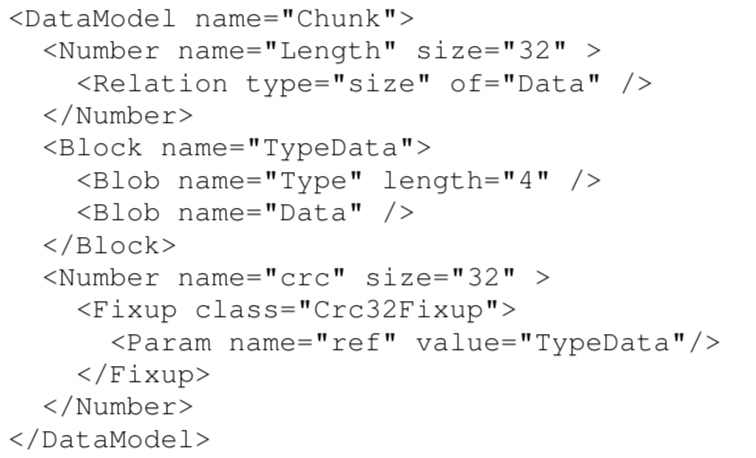
\includegraphics[width=5cm]{images/PeachPit}
      \caption{Data model with a custom format.}
      \label{fig:pit}
\end{figure}
